\section{Top Reconstruction}
\label{sect:top}
To reconstruct the top quarks a special method is used.  
The main features 
of the method are using a $\chi^2$ and mass of the jets. A $\chi^2$ is
constructed based on the known masses of $W$ and top, e.g.
\begin{linenomath}
\begin{equation}
\label{eq:chi2}
\chi^2 = \frac{(M_{2j} - M_W)^2}{\sigma^2_W} + \frac{(M_{3j} - M_t)^2}{\sigma^2_t}; 
\end{equation}
\end{linenomath}
$M_{2j}$ is usually the invariant mass of 2 jets making a $W$ boson, 
but it can also be a heavy single jet. The uncertainty on invariant masses is computed as
\begin{linenomath}
\begin{equation}
\label{eq:sigma}
\sigma_x = \sqrt{\frac{1}{4}\sum_{i} \pod{\frac{\Delta p_i}{p_i}}^2\pod{\frac{\sum_{j \neq i} M_{ij}^2}{M}}^2 + \Gamma_x^2}; 
\end{equation}
\end{linenomath}
where $p_i$ uncertainty is taken as $\frac{\Delta p_i}{p_i} = \frac{100\%}{\sqrt{p_i}}$ and $\Gamma_x$ is the width of $W$ (2.1 GeV) 
and top (10 GeV). Top reconstruction is started by reconstructing all possible $W$'s from either 2 jets (W2j) or 1 heavy jet (W1j).
Solutions are kept only if they have a $\chi^2$ which is less than a fixed maximum value (2 in this analysis) for $W$ in W2j
and in W1j giving the $W$ mass in a small window (80.4 $\pm$ 10.0 GeV/$c^2$). To calculate the $\chi^2$ for W1j, the width ($\Gamma_x$) in 
Equation \ref{eq:sigma} is set equal to 10 GeV/$c^2$. If a heavy jet is in a given mass range and is $b$-tagged, 
it is considered as a coalescence of a $b$ with a jet from $W$ (W1b). The mass window for W1b is set to [40,130] GeV/$c^2$ . 
$\chi^2$ = 1 is assigned to W1b candidates to avoid any systematically decrease of $\chi^2$ for the top combinations containing such objects.
All reconstructed $W$'s are ordered in their $\chi^2$ value. In case of overlapping $W$'s, only the best $\chi^2$ solution is kept. 
In next step, the reconstructed $W$'s are used to reconstruct the top candidates by adding a free jet. To reduce the correlations,
before using the $W$'s, their 4-vector is rescaled to give the correct $W$ mass (80.4 GeV/$c^2$). If there is any overlap between the tops, 
the combination with a correct $b$-tagged jet ($b$+$W$) or a W1b is preferred over the best $\chi^2$ solution. 

\subsection{Performance of the Algorithm}
By efficiency we want to know how many of generated top quarks are found at reconstruction level with “top search” algorithm. Only hadronically decaying top quarks are considered. Efficiency is defined as 

$$\epsilon_{topSearch} = N_{reco-top}^{matched}  / N_{gen-top}^{hadronic}$$

where reconstructed top quarks are matched with generated ones if $\Delta R < 0.1$. The overall results are shown in Table \ref{tbltopreceff}.

\begin{table}[htb]
  \begin{center}
    \begin{tabular}{|c|c|c|c|c|}
      \hline
      \textbf{\#events}  &  \textbf{\#gen-top-hadronic}  &  \textbf{\#rec-top-all}  &  \textbf{\#rec-top-matched}  &  \textbf{Overall efficiency}  \\
      \hline
      1.16 ME          &                        2601  &                   1331  &                   936  &  36\%                  \\
      \hline
    \end{tabular}
    \caption{The total efficiency of the top reconstruction algorithm. The efficiency is defined as the fraction of the generated top quarks which are reconstruted by the top search algorithm.}
    \label{tbltopreceff}
  \end{center}
\end{table}

Efficiency versus different event kinematic variables is studied and the results are shown in Figure \ref{figtopref_eff}. Efficiency is investigated in different jet bins. The probability to find a hadronically decaying top in higher jet multiplicities is higher.

The efficiency of the top reconstruction vs. number of b-tagged jets is also studied. Although there is no constraint for the combination to contain a b-tagged jet, in case of a tagged jet in the top combination, it is preferred over minimum $\chi^2$. Efficiency is stable in Nb-jets bins, as expected. The last bin suffers from low statistics.

As the efficiency versus the top $\pT$ is shown in Figure \ref{figtopref_eff}, If top quarks are “generated” with higher $\pT$, there is a higher probability for them to be reconstructed by our algorithm.

This study shows that efficiency is stable in $\mttwo$ bins, apart from the last two bins which have few entries.

\begin{figure}[htbp] 
\centering
    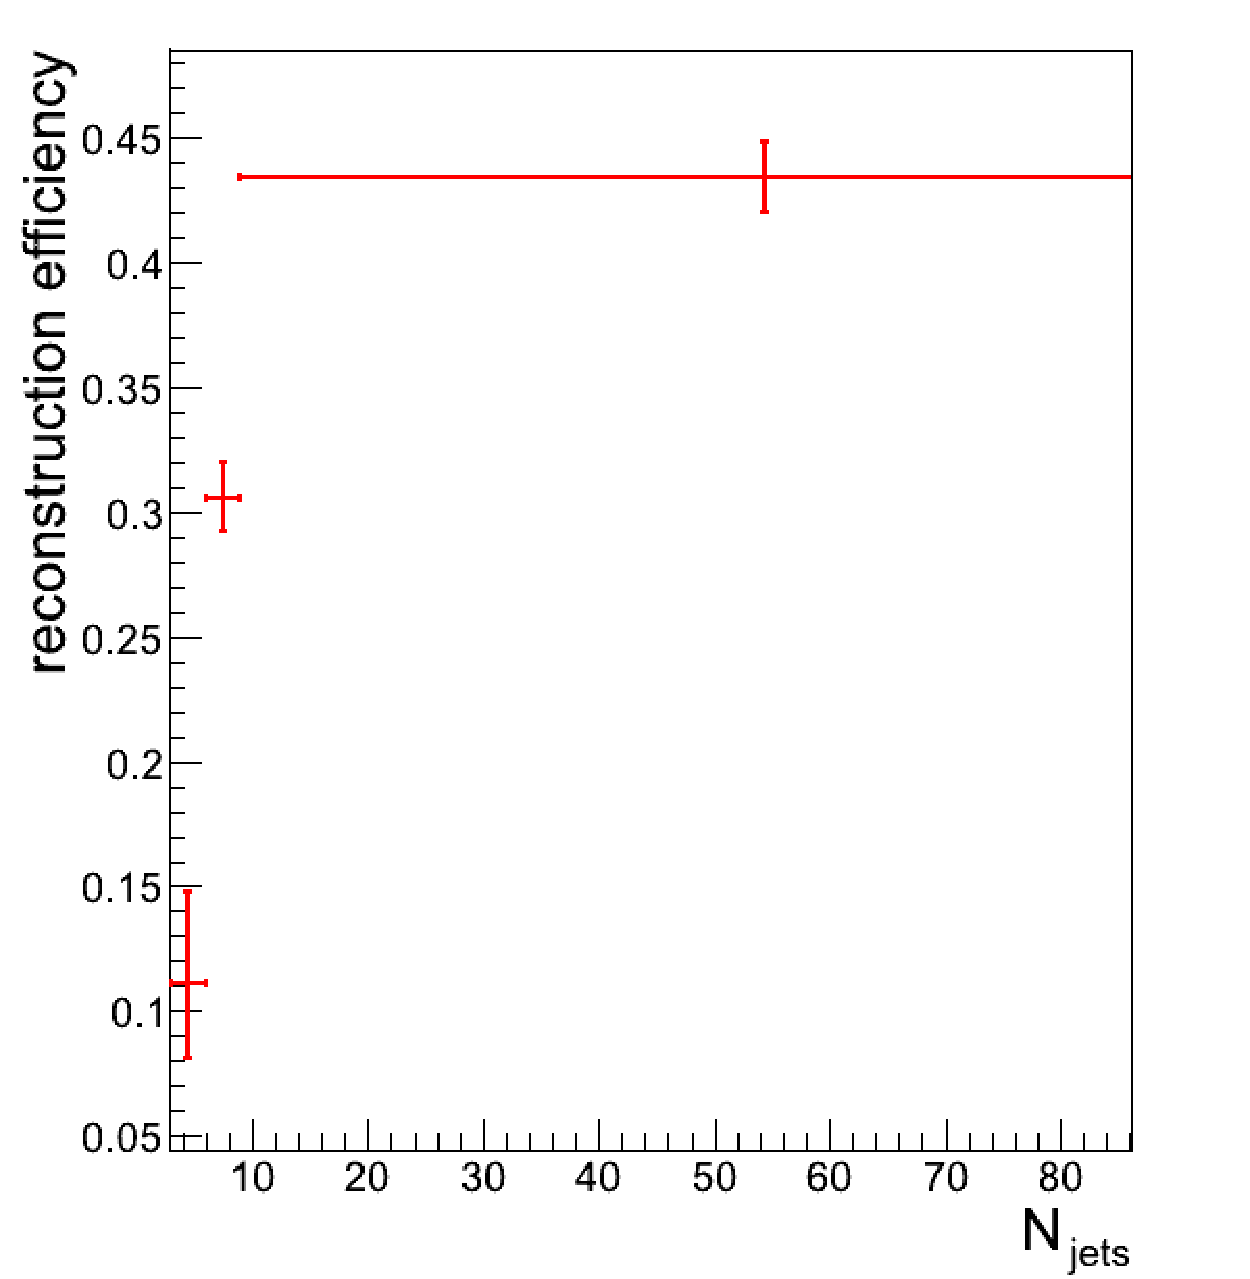
\includegraphics[width=0.3\textwidth]{figs/topNjet.pdf}
    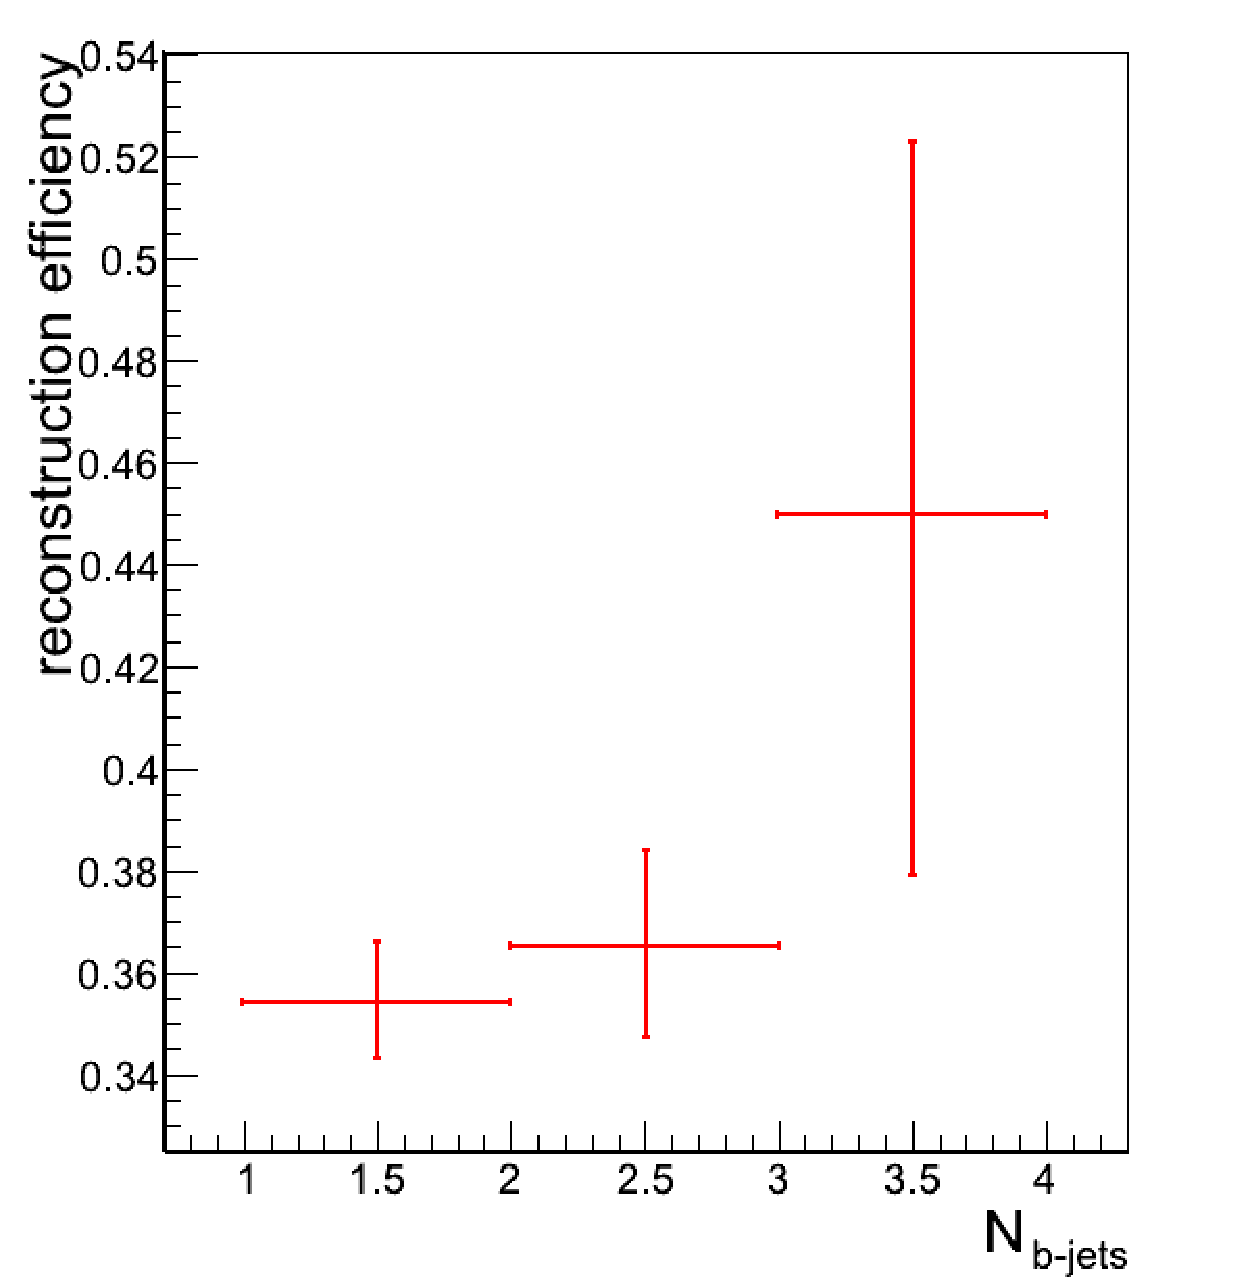
\includegraphics[width=0.3\textwidth]{figs/topNbjet.pdf} \\
    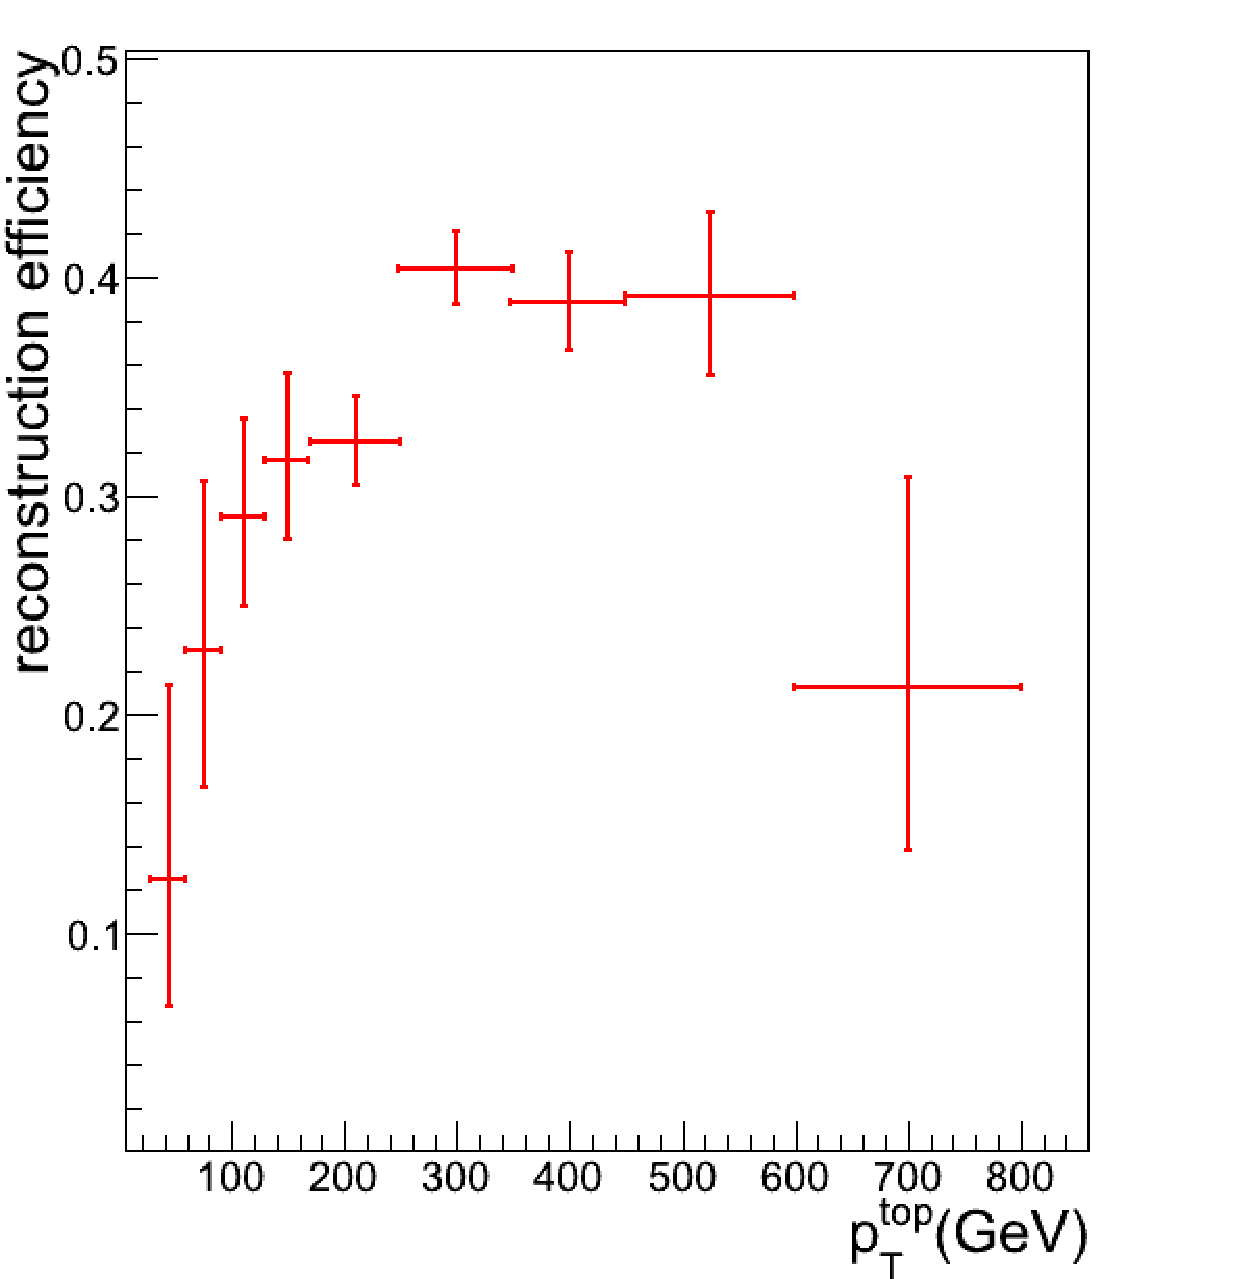
\includegraphics[width=0.3\textwidth]{figs/topPt.pdf}
    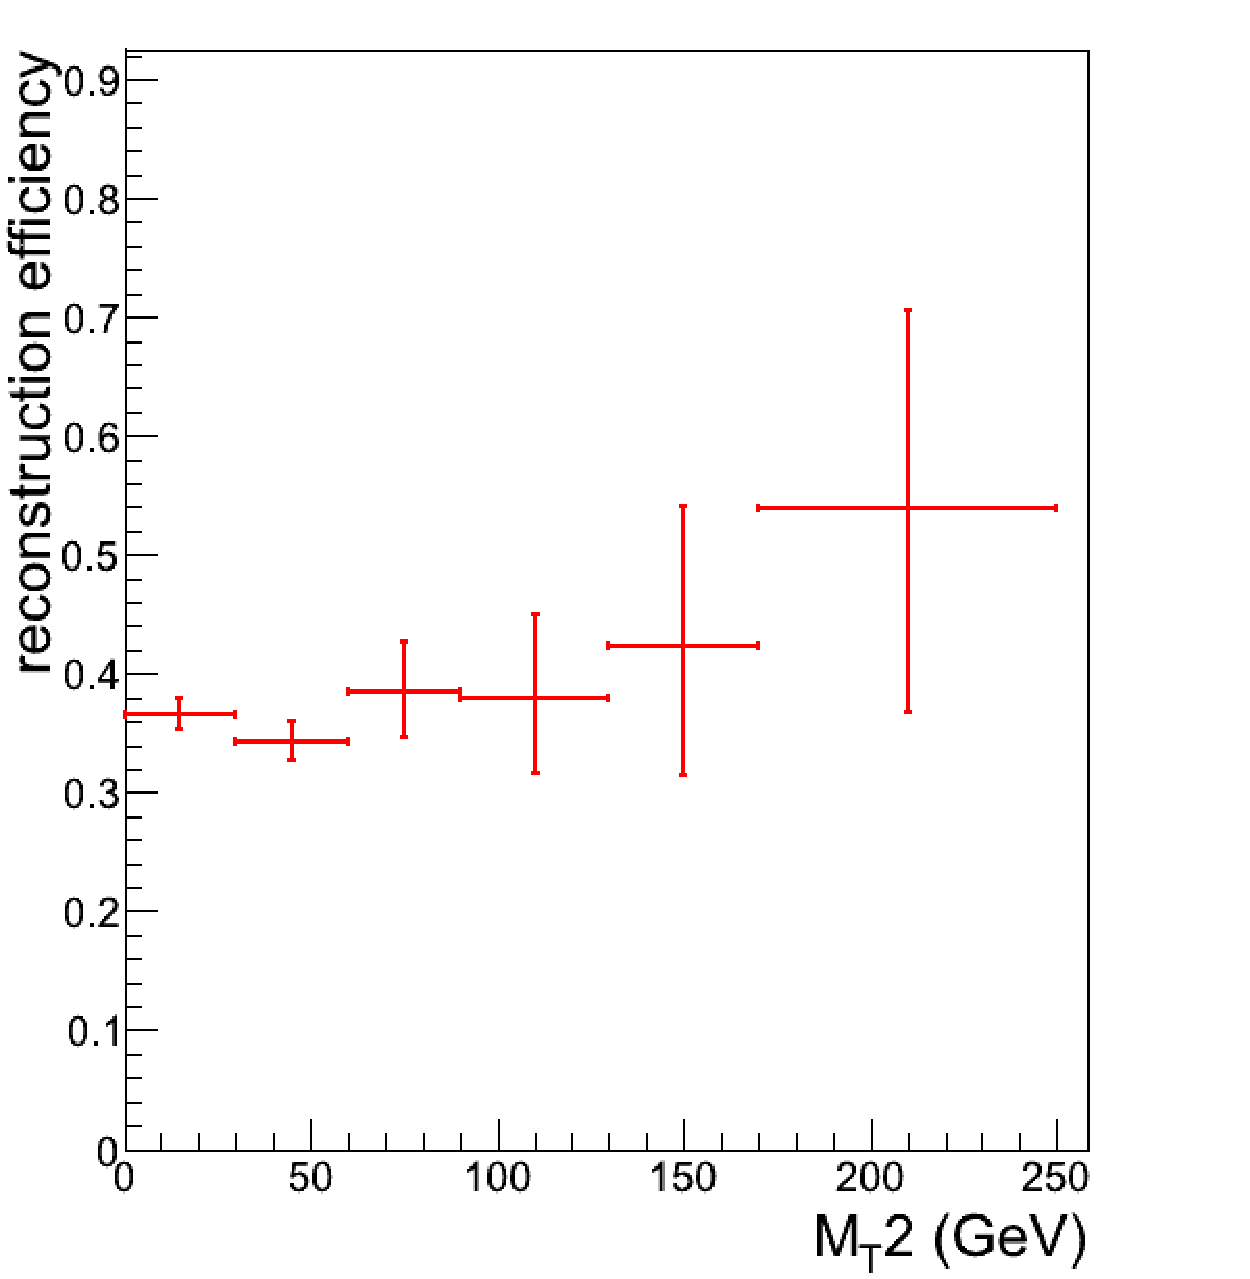
\includegraphics[width=0.3\textwidth]{figs/topMT2.pdf}
    \caption{The efficiency of top reconstruction algorithm vs. number of jets (left) and number of b-tagged jets (right) in the above row and top $\pT$ (left) and $\mttwo$ (right) in the below row are shown.}
    \label{figtopref_eff}
\end{figure}


The fake rate of the top reconstruction algorithm is also studied. Fake Rate, can be defined as the Probability of reconstructing top from each 3 jets in a $W$ + jets event. So the ratio is normalized to the number of jets. The results after applying all MT2b cuts on the WJetsToLNu-HT-400ToInf-8TeV sample are shown in Figure \ref{figtopref_fake}. The studies show that the fake rate value is around $20\%$.


\begin{figure}[htbp] 
\centering
    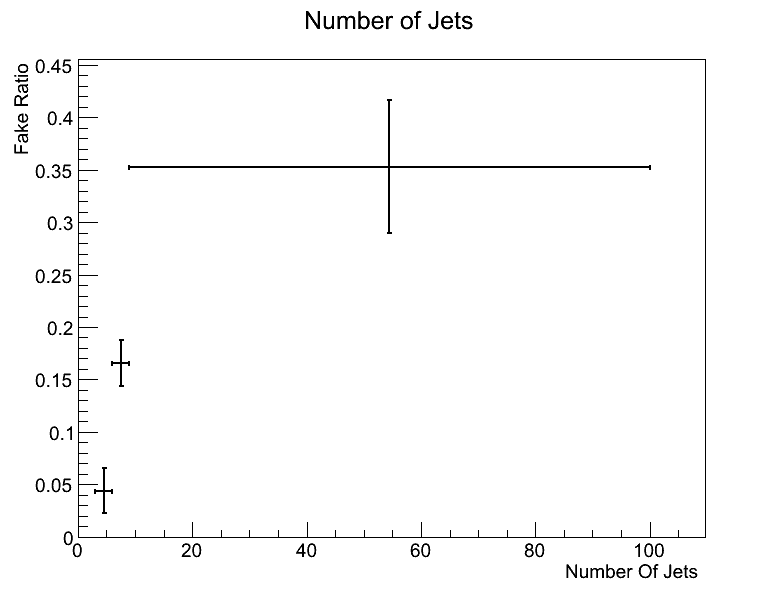
\includegraphics[width=0.3\textwidth]{figs/top_fake_NJets.png}
    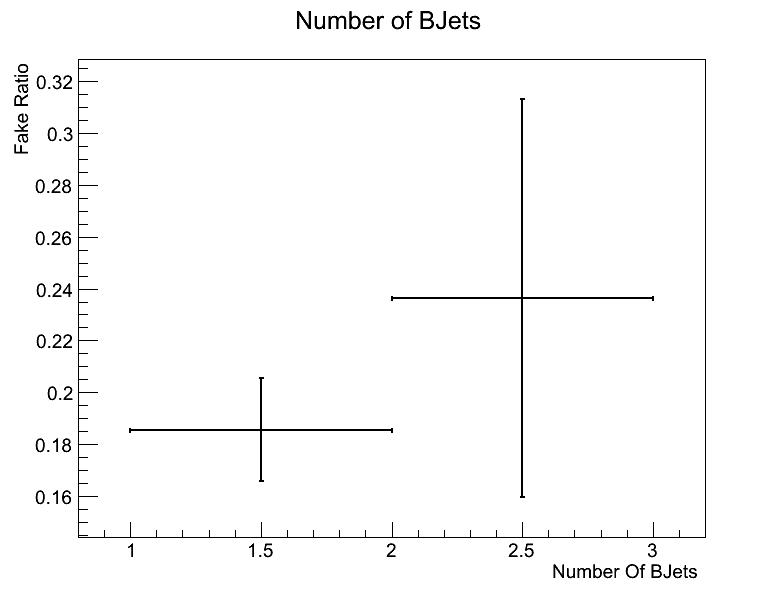
\includegraphics[width=0.3\textwidth]{figs/top_fake_NBJets.png} \\
    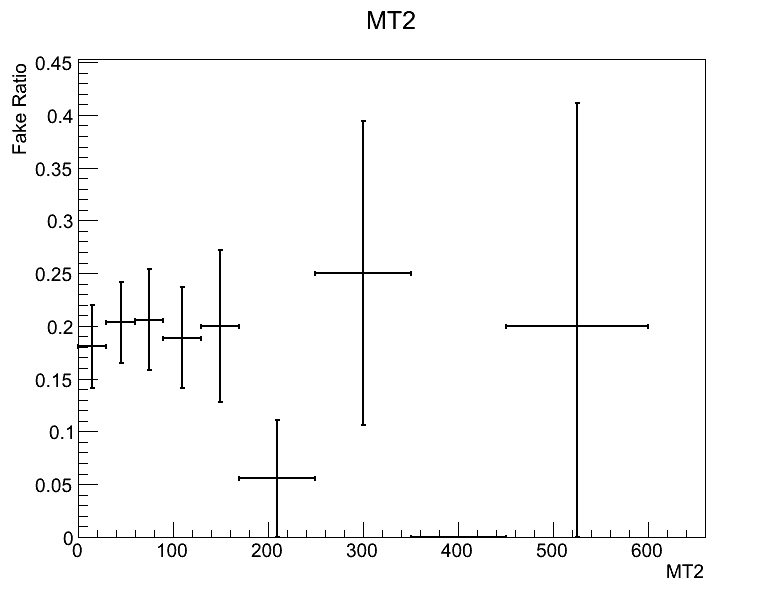
\includegraphics[width=0.3\textwidth]{figs/top_fake_MT2.png}
    \caption{The fake rate of the top reconstruction algorithm vs. number of jets (left) and number of b-tagged jets (right) in the above row and also vs. $\mttwo$ in the below row are shown.}
    \label{figtopref_fake}
\end{figure}
